\begin{frame}{Prior Work: Process Notes}
\protect\hypertarget{prior-work-process-notes}{}
\begin{itemize}
\tightlist
\item
  SiLab Designs have migrated over time

  \begin{itemize}
  \tightlist
  \item
    2007-2011: 130nm
  \item
    2012-Present: 65nm
  \end{itemize}
\item
  Now 28nm is available, but:

  \begin{itemize}
  \tightlist
  \item
    2-4x transistors -\textgreater{} longer simulation, layout,
    verification
  \item
    3x PDK/DRC rules
  \item
    2x cost (8k EUR/mm\^{}2)
  \end{itemize}
\item
  Smaller != better

  \begin{itemize}
  \tightlist
  \item
    Must consider A vs D performance, power, area, cost
  \end{itemize}
\item
  ISSCC trend anecdote: 65nm is still most popular node
\end{itemize}
\end{frame}

\begin{frame}{Prior Work: PLL Designs}
\protect\hypertarget{prior-work-pll-designs}{}
\begin{columns}[T]
\begin{column}{0.48\textwidth}
\textbf{Early DHP PLL, in 90nm, later ported to 65nm}
\includegraphics{../images/dhptpll.png}
\end{column}

\begin{column}{0.48\textwidth}
\textbf{Early RD53 PLL, 65nm, later grew to 600ux150u}
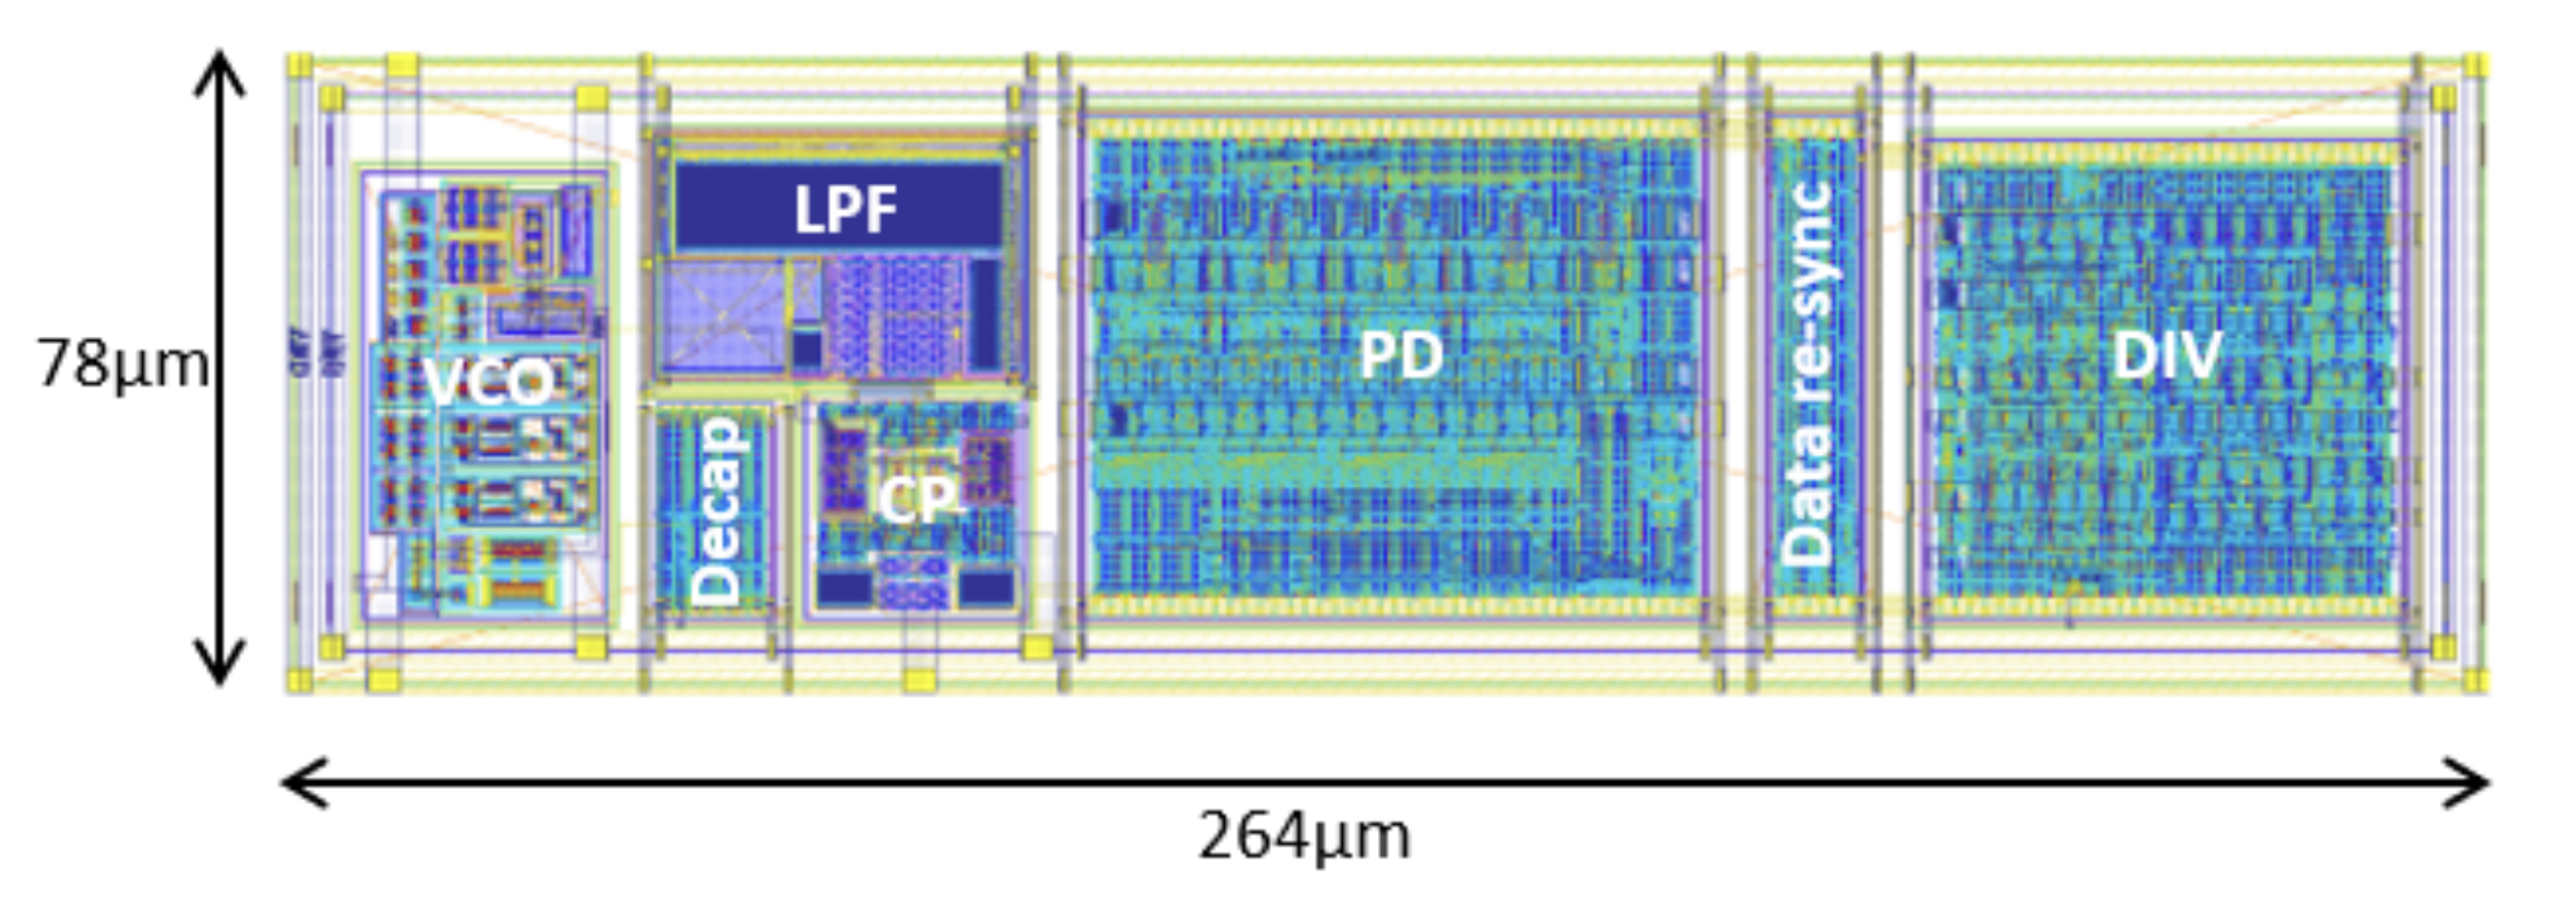
\includegraphics{../images/rd53pll.jpeg}
\end{column}
\end{columns}

\begin{longtable}[]{@{}llllll@{}}
\toprule()
Design & Fin(Hz) & Fout(Hz) & Jitter(s) & Power(W) & TID(Rad) \\
\midrule()
\endhead
DHP & 80M & 1.6G & 20p & 1.25m VCO & 20M \\
RD53 & 80M & 1.28G & 5p & 6.5m & 500M \\
\bottomrule()
\end{longtable}
\end{frame}

\begin{frame}{Generators: What \& Why}
\protect\hypertarget{generators-what-why}{}
\begin{columns}[T]
\begin{column}{0.48\textwidth}
\begin{itemize}
\tightlist
\item
  Common analog `IP' (IBias, VRef, PLL, IO, ADC, DAC)
\item
  Portable and/or parallel design (65nm or 28nm?)
\item
  Record design method/intent (Why this W/L?)
\item
  Faster modification (e.g.~layout ECOs)
\item
  General-purpose tooling (Python, C++, YAML)
\end{itemize}
\end{column}

\begin{column}{0.48\textwidth}
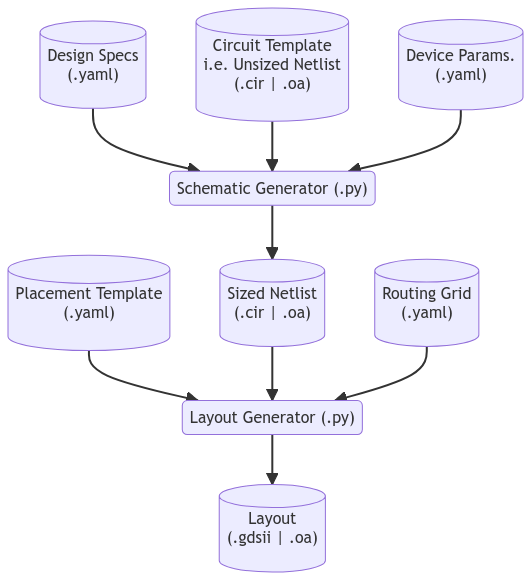
\includegraphics{../images/flow.png}
\end{column}
\end{columns}
\end{frame}

\begin{frame}{Generators: Procedural}
\protect\hypertarget{generators-procedural}{}
\begin{columns}[T]
\begin{column}{0.48\textwidth}
\begin{itemize}
\tightlist
\item
  ``White Box'' mechanistic modeling \& optimization
\item
  Capture known solution to known problem
\item
  Limited simulation for parameters -\textgreater{} Fast
\item
  Top-to-bottom: `feedforward'
\end{itemize}
\end{column}

\begin{column}{0.48\textwidth}
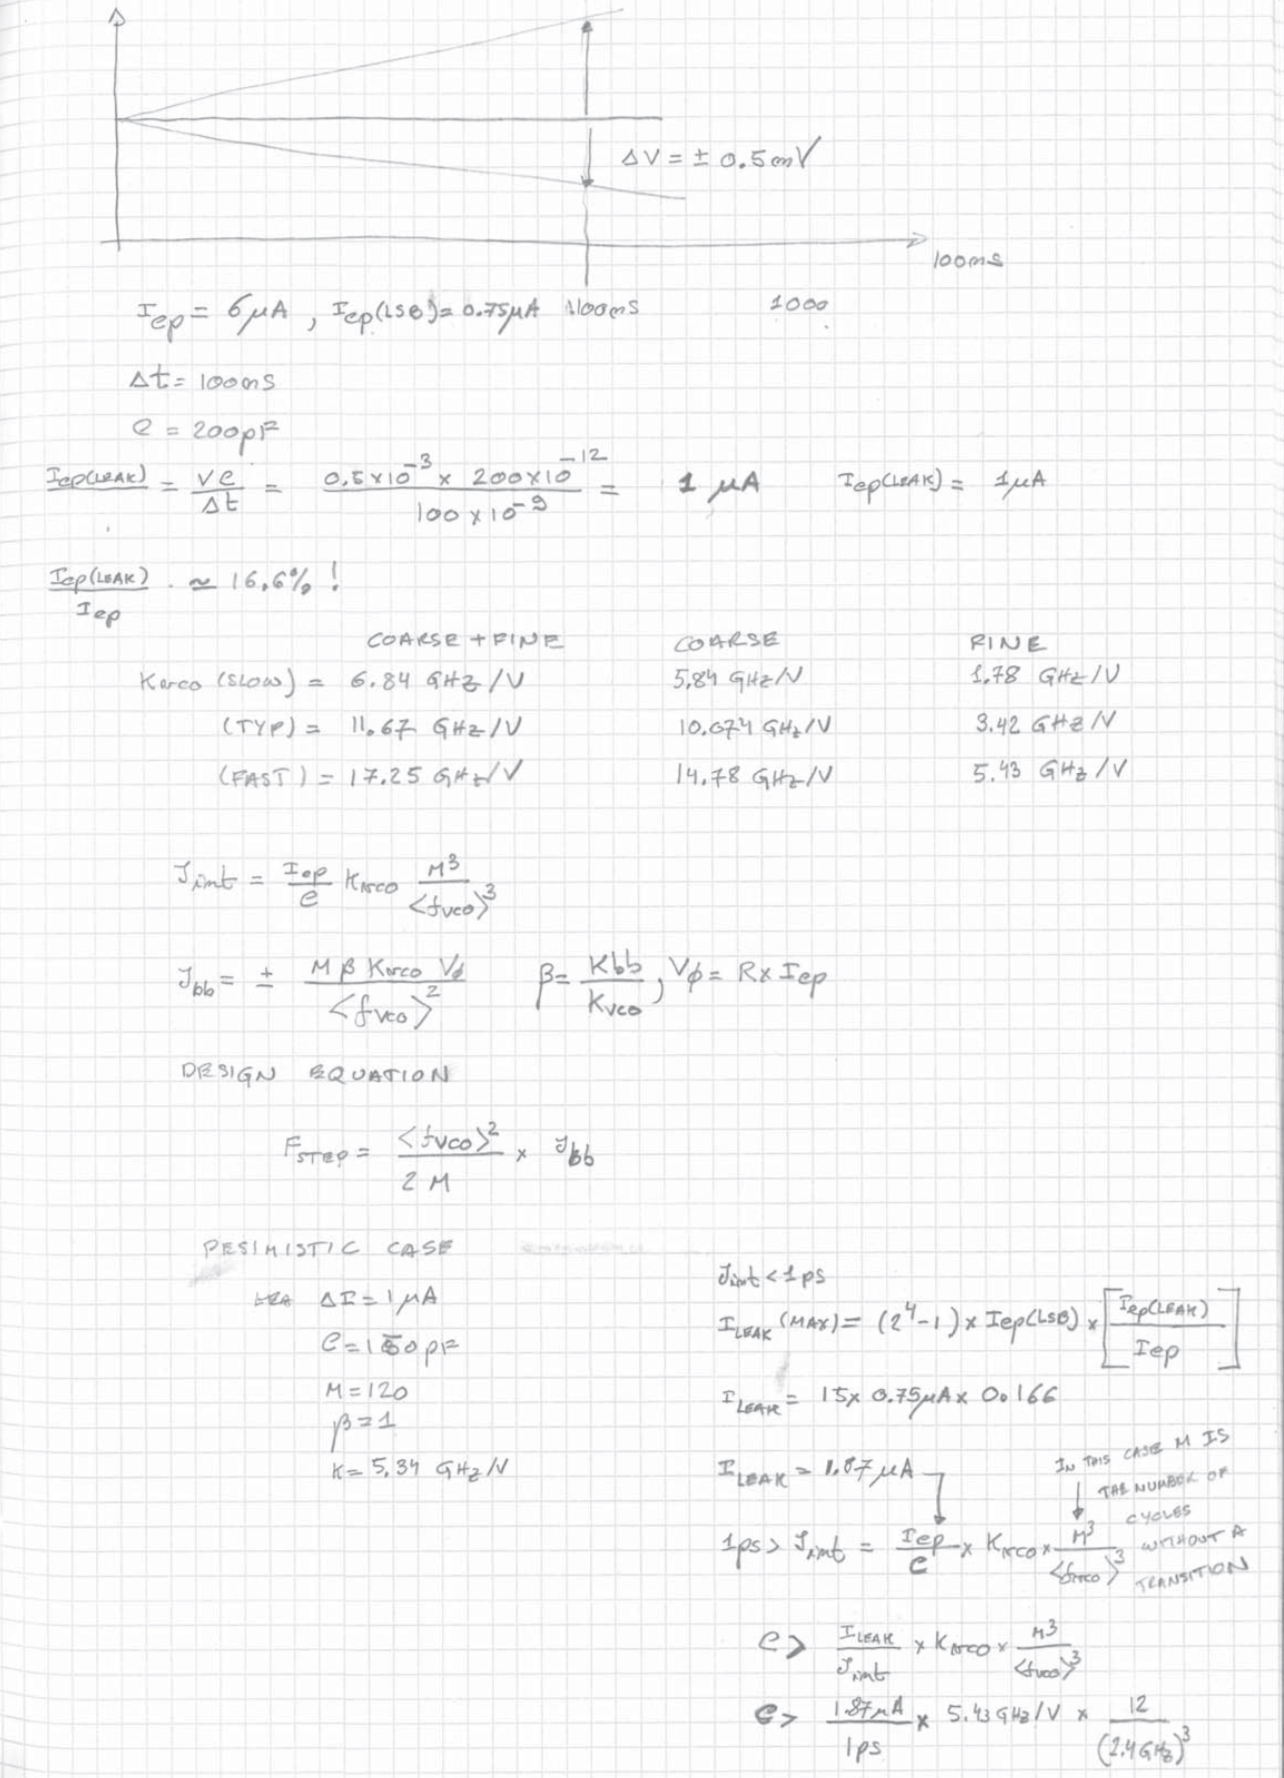
\includegraphics{../images/IMG_1500.jpeg} \emph{Rare `procedural
generator' specimen, circa 2013}
\end{column}
\end{columns}
\end{frame}

\begin{frame}{Generators: Synthesis}
\protect\hypertarget{generators-synthesis}{}
\begin{columns}[T]
\begin{column}{0.48\textwidth}
\begin{itemize}
\tightlist
\item
  ``Black Box'' optimization; give computer constraints and objective
  and let it explore
\item
  More formally: \emph{Metaheuristic optimization}

  \begin{enumerate}
  \tightlist
  \item
    Produce a set of candidates
  \item
    Evaluate via simulation -\textgreater{} Slow!
  \item
    Retain best performing
  \item
    Iterate if necessary: `feedback'
  \end{enumerate}
\end{itemize}
\end{column}

\begin{column}{0.48\textwidth}
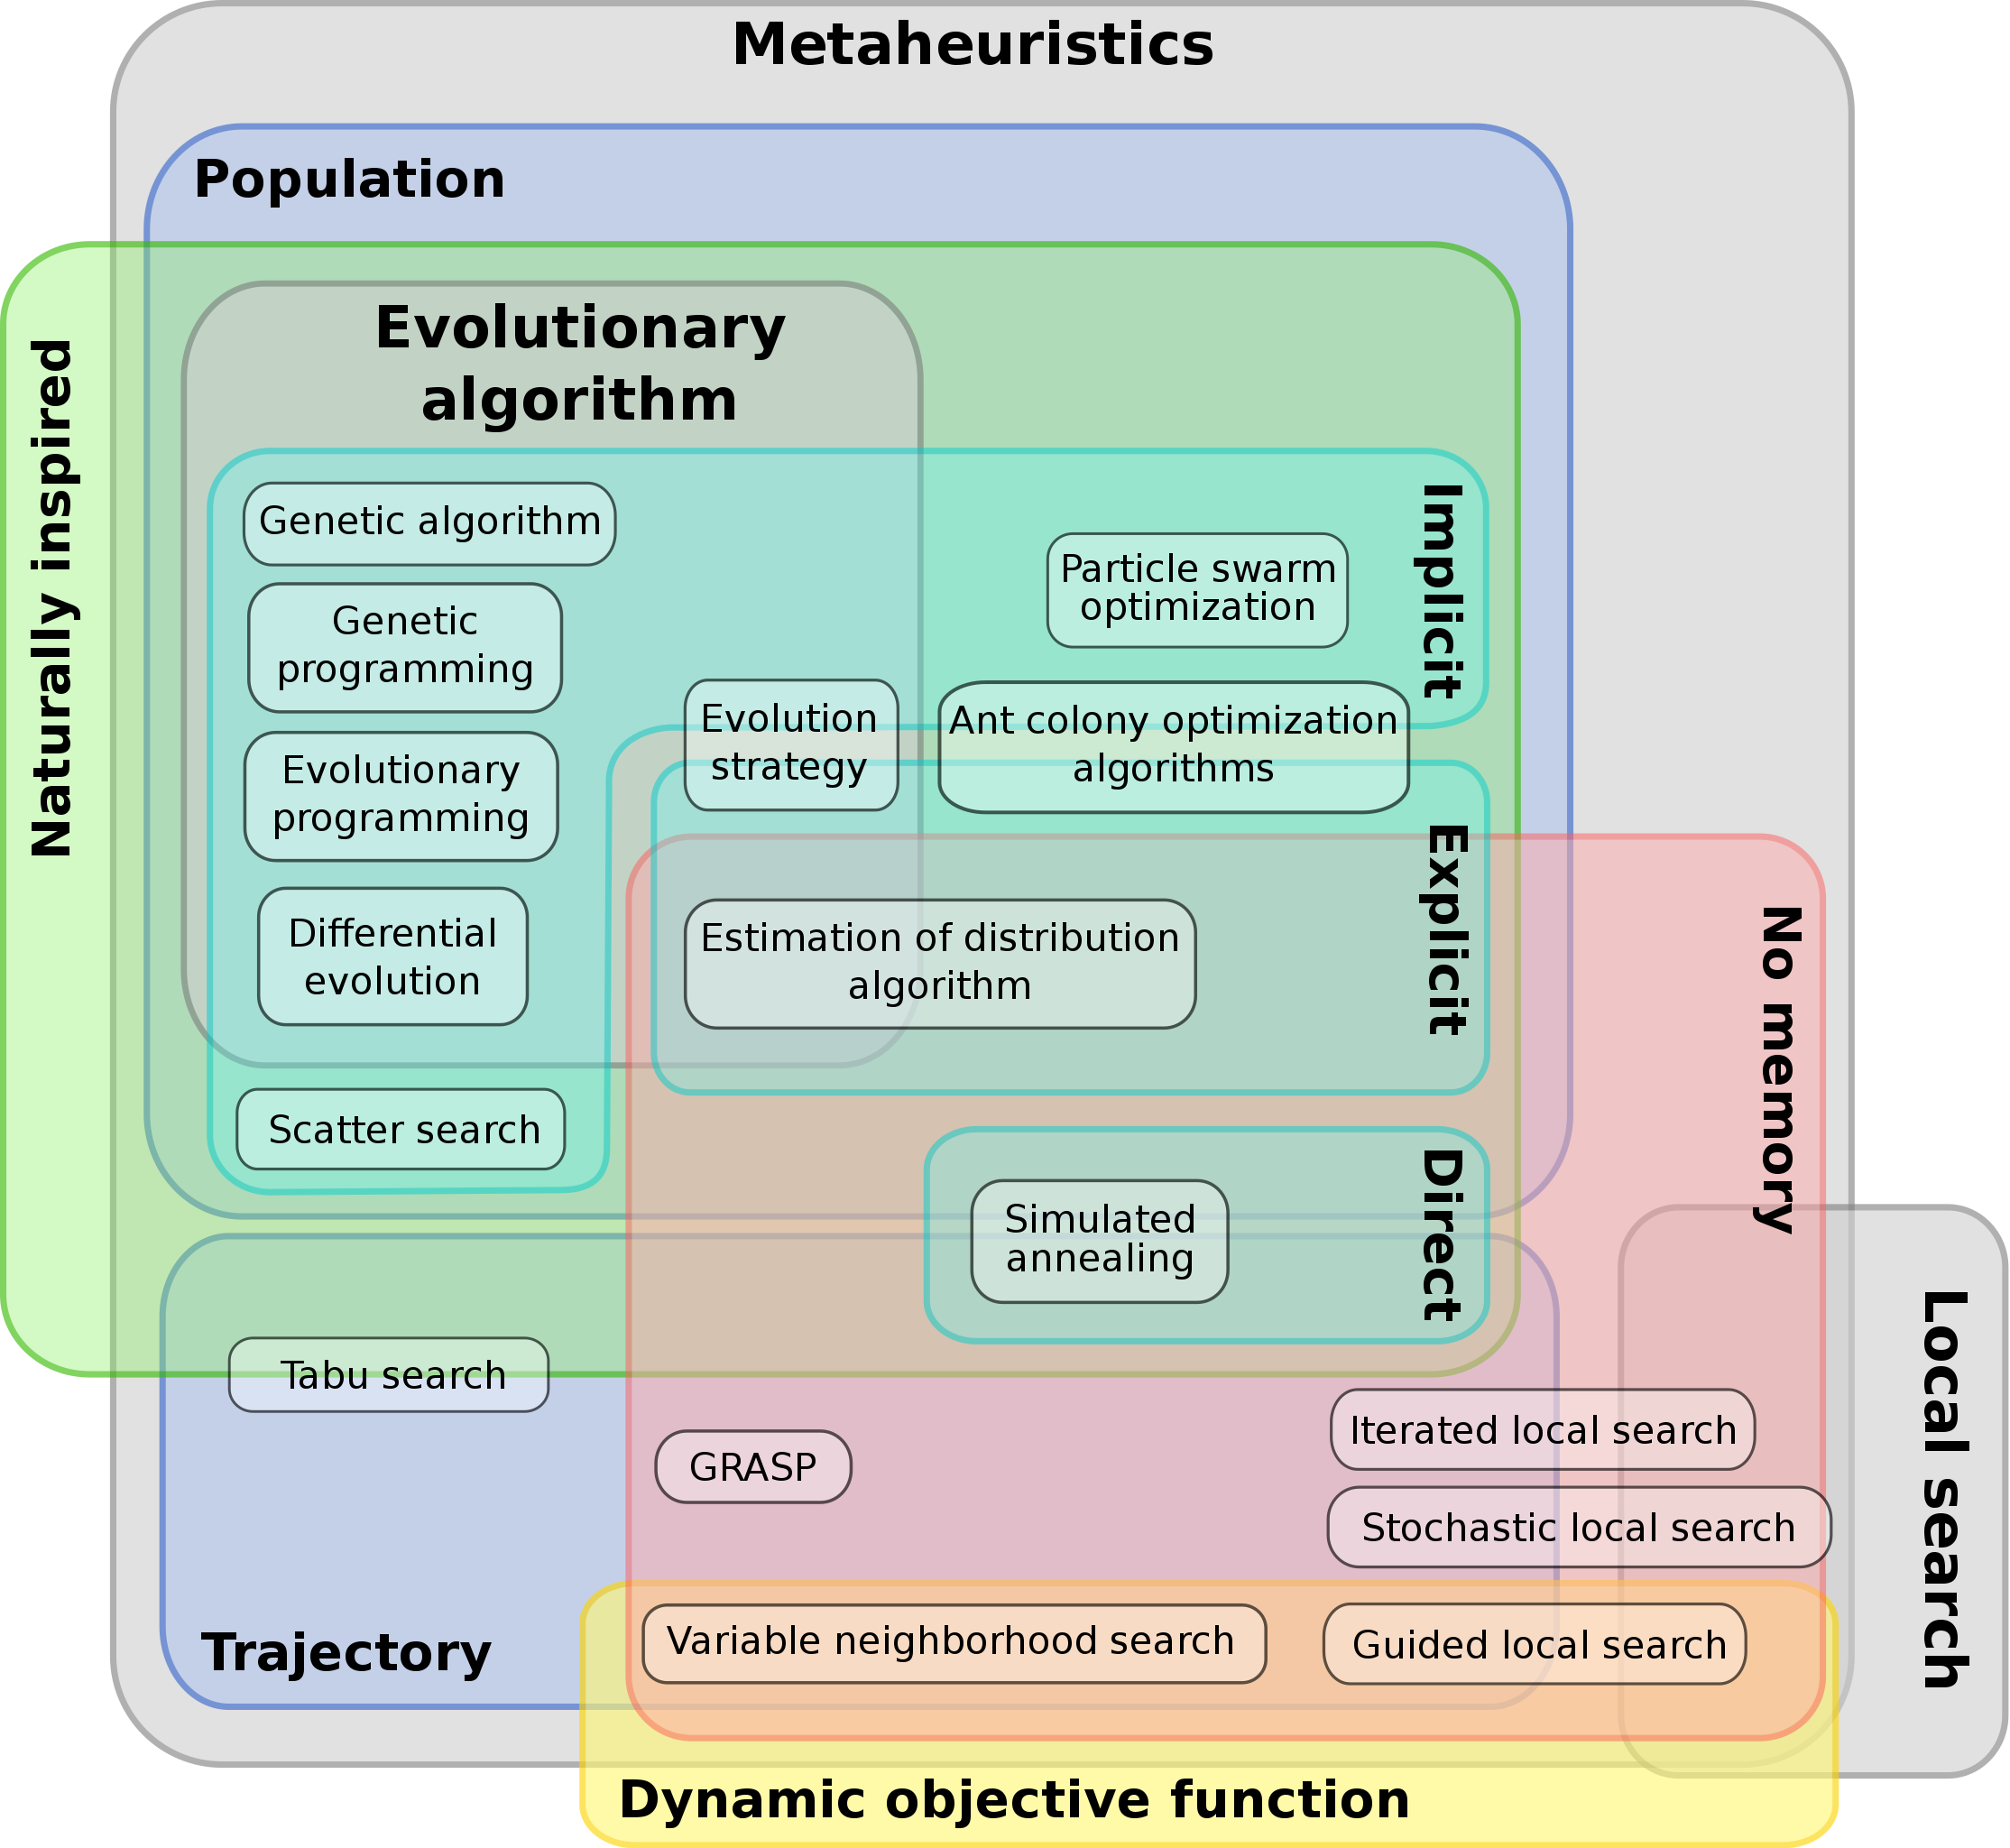
\includegraphics{../images/IMG_1501.png}
\url{https://en.m.wikipedia.org/wiki/Metaheuristic}
\end{column}
\end{columns}
\end{frame}

\begin{frame}{Generators: When to use which type?}
\protect\hypertarget{generators-when-to-use-which-type}{}
\begin{itemize}
\tightlist
\item
  Sizing vs Layout: Sizing can be either; or combination, analog layout
  should probably always be procedural
\item
  Linear vs Non-Linear
\item
  System vs device
\item
  Regular vs non-regular: more common in 28nm!!
\item
  Schematic vs layout
\end{itemize}
\end{frame}

\begin{frame}{Generators: Dos and don'ts}
\protect\hypertarget{generators-dos-and-donts}{}
\begin{itemize}
\tightlist
\item
  \textbf{DO} create a deterministic generator (e.g.~avoid random
  optimization convergence)
\item
  \textbf{DO} use constraints (specs, schem/layout templates, routing
  grids, abstract PDK/DRC)
\item
  \textbf{DO} work in GP languages: flexibility, shared w/ real-world
  testing, readability, source control, sharing w/o NDA
\item
  \textbf{DO} combine the procedural + synthesis (Mimics what designers
  already do intuitive)
\item
  \textbf{DO} partition generator code by cell view
\item
  \textbf{DON'T} hide method in opaque neural networks (human or
  machine)

  \begin{itemize}
  \tightlist
  \item
    Over-constrained procedural not reusable and ignores useful
    abstraction (e.g.~drawing raw GDSII)
  \item
    Under-constrained statistical approach time-consuming and
    meaningless, (e.g.~unsupervised learning
  \end{itemize}
\item
  \textbf{DON'T} use for one-off/unique blocks or top-level
\item
  \textbf{DON'T} expect SOTA performance, power, area
\end{itemize}
\end{frame}

\begin{frame}{Generators: Survey of Tools}
\protect\hypertarget{generators-survey-of-tools}{}
\begin{itemize}
\tightlist
\item
  \textbf{PCell \& PyCell}: W\&L -\textgreater{} OA Layout+BSIM6, SKILL
  or Python/OA
  \href{https://www.synopsys.com/cgi-bin/pycellstudio/req1.cgi}{Site}
  \href{https://arxiv.org/pdf/1607.00859.pdf}{Paper}
\item
  \textbf{BAG}: OA Schem Template -\textgreater{} OA Schem, Python+SKILL
  \href{https://bag3-readthedocs.readthedocs.io/en/latest/workspaces.html}{Docs}
  \href{https://github.com/ucb-art/bag/tree/without_OA}{Code}
\item
  \textbf{Hdl21} / \textbf{Layout21}:
  \href{https://github.com/dan-fritchman/Hdl21}{Code}
\item
  \textbf{gdstk(prev. gdspy)}: Python -\textgreater{} GDSII, Python
  \href{https://github.com/heitzmann/gdstk}{Code}
\item
  \textbf{MAGICAL}: \href{https://github.com/magical-eda/MAGICAL}{Code}
\item
  \textbf{ALIGN}: Netlist -\textgreater{} GDSII, Python, FOSS
  \href{https://github.com/ALIGN-analoglayout/ALIGN-public}{Code}
\item
  \textbf{Anagen} - Closed source, Infineon
  \href{https://m.youtube.com/watch?v=IzJbVG-FHJc}{Pres}
\item
  \textbf{IIP Framework}: Fraunhaufer IIS, Closed source,
  \href{https://publica-rest.fraunhofer.de/server/api/core/bitstreams/c8d21689-7db1-405f-b1b8-a2298eedf7a3/content}{Pres}
  \href{https://www.eas.iis.fraunhofer.de/en/business_areas/efficient_electronics/automation-analog-design.html}{Web}
  \href{https://ieeexplore.ieee.org/document/7520725}{Paper}
\item
  \textbf{LayGO2}:
\item
  \textbf{FASoC}: UMichigan \href{https://fasoc.engin.umich.edu/}{Link}
  \href{https://github.com/idea-fasoc/fasoc}{Git}
  \href{https://ieeexplore.ieee.org/document/9344104/authors\#authors}{Paper}
\item
  \textbf{OpenFASoC}: UMichigan
  \href{https://openfasoc.readthedocs.io/en/latest/getting-started.html}{Docs}
  \href{https://github.com/idea-fasoc/OpenFASOC}{Git}
\end{itemize}
\end{frame}

\begin{frame}{Next Steps: Application}
\protect\hypertarget{next-steps-application}{}
\begin{columns}[T]
\begin{column}{0.48\textwidth}
\begin{itemize}
\tightlist
\item
  Phase/Freq. Detector: Depending on Linear, Bang-Nonlinear. Noise
  Margin Suppresses Voltage Noise, mostly digital, this is a irregular
  but structural block, low gate/stage block, so this is best followed
  via a strictly procedural generation for schematic and layout. Can
  likely build from standard cells. Jitter does matter though.
\item
  Charge Pump: functional
\item
  Low Pass Filter: Passive, and so can be considered linear quite
  easily. Relatively straiforward to solved with procedural sizing and
  layout.
\item
  Volt. Controlled Oscillator: Dominant source of jitter, can be very
  nonlinear
\item
  Divider: Straightforward for synchronous design, similar to PFD, take
  advantage of noise noise margin intrinsic to nonlinear operation, just
  pay attention to layout parasitic, jitter
\end{itemize}
\end{column}

\begin{column}{0.48\textwidth}
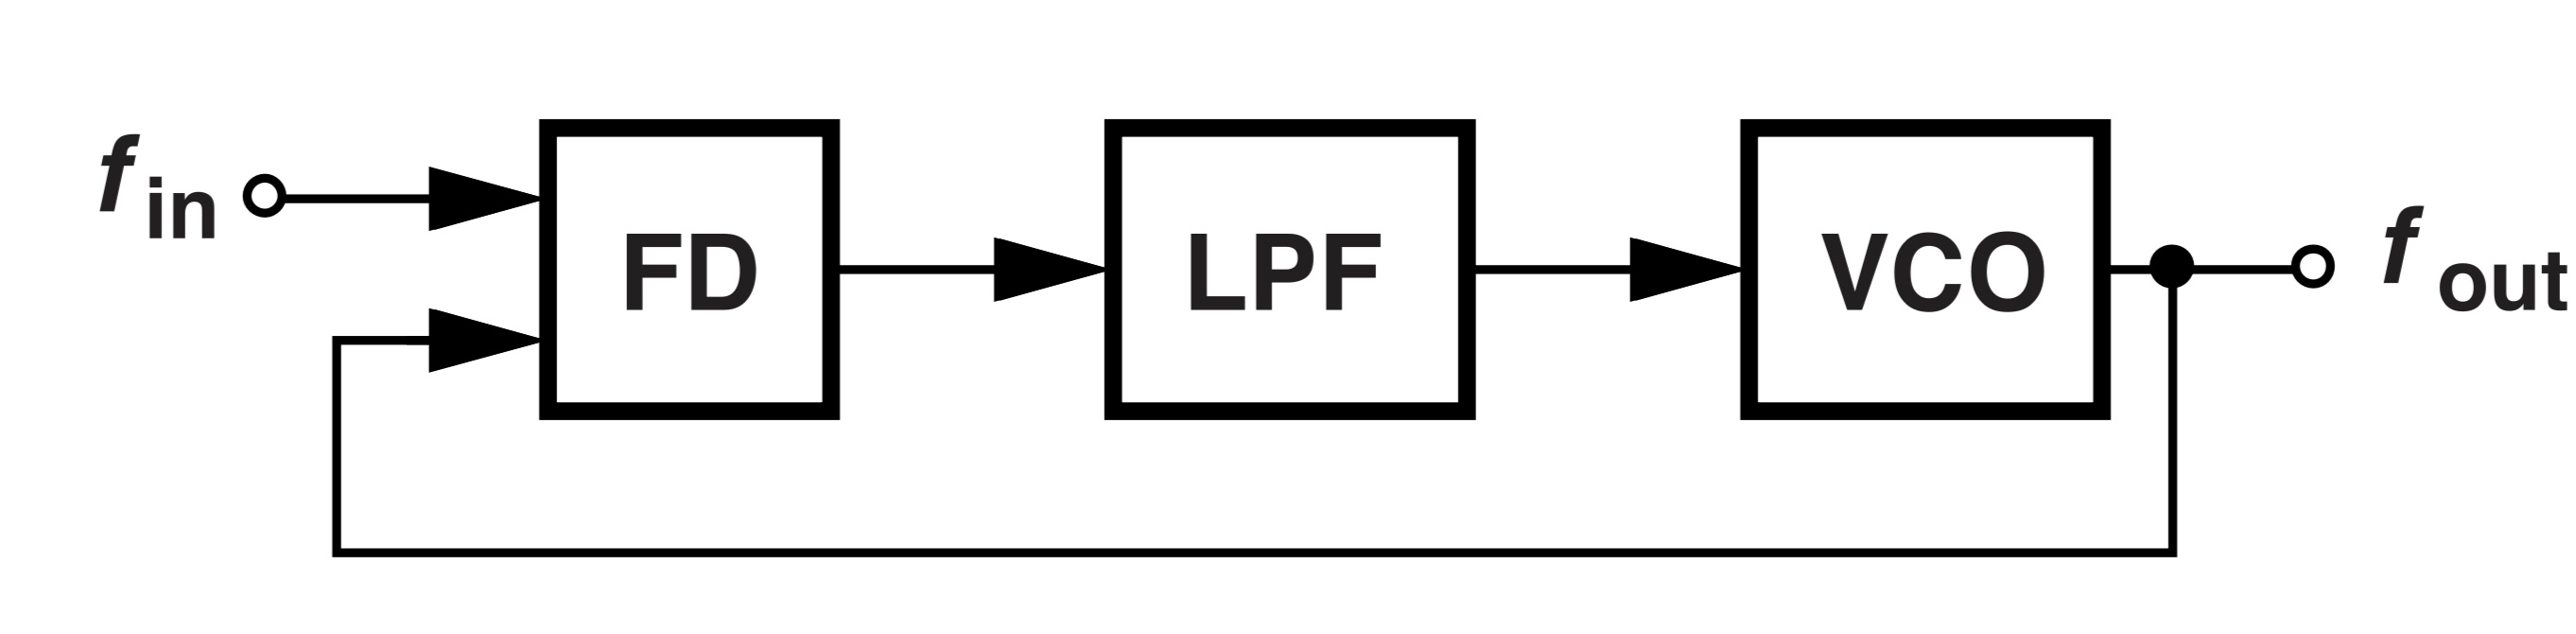
\includegraphics{../images/IMG_1502.jpeg}

\href{https://doi.org/10.1017/9781108626200}{B. Razavi, Design of CMOS
Phase-Locked Loops}
\end{column}
\end{columns}
\end{frame}

\begin{frame}{Next Steps: Timeline}
\protect\hypertarget{next-steps-timeline}{}
\begin{itemize}
\tightlist
\item
  Design generator that is 28 nm + 65 nm compatible
\item
  TSMC 28 nm submission of demonstrator PLL via Europractice
\item
  Apply generator concepts to new FE designs
\end{itemize}

\begin{block}{Potential Issues}
\protect\hypertarget{potential-issues}{}
\begin{itemize}
\tightlist
\item
  OpenAccess \& Cadence
\item
  Environment setup
\item
  Alternate abstraction to learn (pro \& con)
\end{itemize}
\end{block}
\end{frame}
